% !TEX program = lualatex

%The Aspectration can be 4:3 (43) and 16:9 (169)
\documentclass[12pt, aspectratio=169, usepdftitle=false]{beamer}
% \documentclass[12pt, aspectratio=169, usepdftitle=false, handout]{beamer}

\usepackage[ngerman]{babel}
\usepackage{marvosym}
\usepackage{pifont}
\usepackage{pgfpages} 
\usepackage{ifthen}
\usepackage{ragged2e}

\usepackage{ubo_tex_beamer/uni-template}
\apptocmd{\frame}{}{\justifying}{} % Allow optional arguments after frame.
% SET TITLE
%----------------------------
\MainTitle{Vertiefungskurs Python}
\SubTitle{\ }

% SET AUTHOR
%----------------------------
\AuthorName{Chris Geron}
\AuthorEmail{s6chgero@uni-bonn.de}
\AuthorInformation{Institut für Informatik}

% SET EVENT-INFORMATION
%----------------------------
\Eventname{Vertiefungskurs Python}
\City{Universität Bonn}
\Date{SoSe 2023}

% Drucke Gitversion
\renewcommand{\printgitversion}{true}
% Drucke Dateinamen
\renewcommand{\printfilename}{true}


% custom packages

\lstset{ backgroundcolor=\color{colororange!5} }

% Include pictures made in inkscape:
\newcommand{\inputhack}{\input}        % Rename \input, so that a very simple awk-skript can merge all tex-files.
\graphicspath{{images/}}               % Set path of the pictures. This is used by the pdf_tex-files generated by inkscape.
\newcommand{\inkpic}[2][\columnwidth]{%
  \def\svgwidth{#1}%
  \inputhack{images/#2.pdf_tex}%
}

\newcommand{\tb}[1]{\textbf{#1}}
\newcommand{\extrainfo}{\begin{textblock}{1}(14.4,.3)\hfuzz=\maxdimen
\includegraphics[width=1.3cm]{images/extra_info.pdf}\end{textblock}}
\newtheorem{defi}{}


\usepackage{textpos}
\setlength{\TPHorizModule}{1cm}
\setlength{\TPVertModule}{1cm}

\newcommand\crule[1][black]{\textcolor{#1}{\rule{2cm}{2cm}}}
\newcommand{\arroworange}{\color{colororange}\Large\MVRightarrow}
\newcommand{\arrowyellow}{\color{coloryellow}\Large\MVRightarrow}
\newcommand{\arrowblue}{\color{colorblue}\Large\MVRightarrow}

\newcommand{\cmark}{\ding{51}}%
\newcommand{\xmark}{\ding{55}}%


\newcommand{\mcO}{\mathcal{O}}


\newcommand{\umlkeyword}[1]{{\color{black}\guillemotleft{}\lpl{#1}\guillemotright{}}}


\newcommand{\shrug}[1][]{%
\begin{tikzpicture}[baseline,x=0.8\ht\strutbox,y=0.8\ht\strutbox,line width=0.125ex,#1]
\def\arm{(-2.5,0.95) to (-2,0.95) (-1.9,1) to (-1.5,0) (-1.35,0) to (-0.8,0)};
\draw \arm;
\draw[xscale=-1] \arm;
\def\headpart{(0.6,0) arc[start angle=-40, end angle=40,x radius=0.6,y radius=0.8]};
\draw \headpart;
\draw[xscale=-1] \headpart;
\def\eye{(-0.075,0.15) .. controls (0.02,0) .. (0.075,-0.15)};
\draw[shift={(-0.3,0.8)}] \eye;
\draw[shift={(0,0.85)}] \eye;
% draw mouth
\draw (-0.1,0.2) to [out=15,in=-100] (0.4,0.95); 
\end{tikzpicture}}


\usepackage{forest}
\forestset{
  default preamble={
    for tree={
      circle,
      draw,
      thick,
      color=black,
      fill=colororange!25,
      text=black,
      minimum size=1.5ex,
      edge+={draw=black, thick},
    },
    delay={
      where content={}{% just the empty nodes
        phantom,
      }{},
    },
  }
}

\tikzset{
  node/.style={
    text=black,
    draw=black,
  },
  tri/.style={
    draw=black,
    isosceles triangle,
    isosceles triangle apex angle=22,
    shape border rotate=90,
    inner sep=0.1pt,
    minimum width=0.5cm,
  }
}

% UML Diagramme
\let\attribute\relax % Workaround needed for old pgf-umlcd-packages
\usepackage[simplified]{pgf-umlcd}
\usetikzlibrary{arrows, arrows.meta}
\providecommand{\umltextcolor}{}
\providecommand{\umlfillcolor}{}
\providecommand{\umldrawcolor}{}
\renewcommand{\umltextcolor}{colorblue}
\renewcommand{\umlfillcolor}{coloryellow!20}
\renewcommand{\umldrawcolor}{coloryellow}

\tikzstyle{classdiag} = [
  every node/.style = {font=\footnotesize}
]

\tikzset{
  template parameter/.style={
    append after command={
      node [draw, densely dashed, umlcolor, font=\ttfamily]
        at (\tikzlastnode.north east)
        {#1}
    }
  }
}

\tikzstyle{umlnode} = [
  font=\footnotesize\bfseries,
  draw=coloryellow,
  fill=coloryellow!20,
  text width=3.5cm,
  align=center,
  anchor=north west
]

\tikzstyle{umlarrow} = [
  thick,
  draw=coloryellow
]

\newcommand{\todo}[1]{\textbf{\color{red}\ #1 \ }}

\newcommand{\framecardfragen}{
  \framecardorange{
    \utext{Haben Sie Fragen?}
  }
}


% Socket und Plug
\makeatletter

\pgfdeclareshape{rotsocket}
{
  \inheritsavedanchors[from=circle] % this is nearly a circle
  \inheritanchorborder[from=circle]
  \inheritanchor[from=circle]{north}
  \inheritanchor[from=circle]{north west}
  \inheritanchor[from=circle]{north east}
  \inheritanchor[from=circle]{center}
  \inheritanchor[from=circle]{west}
  \inheritanchor[from=circle]{east}
  \inheritanchor[from=circle]{mid}
  \inheritanchor[from=circle]{mid west}
  \inheritanchor[from=circle]{mid east}
  \inheritanchor[from=circle]{base}
  \inheritanchor[from=circle]{base west}
  \inheritanchor[from=circle]{base east}
  \inheritanchor[from=circle]{south}
  \inheritanchor[from=circle]{south west}
  \inheritanchor[from=circle]{south east}
%   \inheritbackgroundpath[from=circle]
  \foregroundpath{
    \centerpoint%
    \pgf@xc=\pgf@x%                                                                                                                   \pgf@xc = x value of centerpoint
    \pgf@yc=\pgf@y%                                                                                                                   \pgf@yc = y value of centerpoint
    \pgfutil@tempdima=\radius%                                                                                              \pgfutil@tempdima = radius
    \pgfmathsetlength{\pgf@xb}{\pgfkeysvalueof{/pgf/outer xsep}}%                                                                     \pgf@xb = outer xsep
    \pgfmathsetlength{\pgf@yb}{\pgfkeysvalueof{/pgf/outer ysep}}%                                                                     \pgf@yb = outer ysep
    \pgfmathsetmacro{\pgf@socket@rotate}{\pgfkeysvalueof{/tikz/socket rotate}}%                                            \pgf@socket@rotate = socket rotate
    \ifdim\pgf@xb<\pgf@yb%
      \advance\pgfutil@tempdima by-\pgf@yb%
    \else%
      \advance\pgfutil@tempdima by-\pgf@xb%
    \fi%
    % Background color
    \pgfpathmoveto{\pgfpointadd{\pgfqpoint{\pgf@xc}{\pgf@yc}}{\pgfqpoint{-0.65\pgfutil@tempdima}{ 0.5\pgfutil@tempdima}}}
    \pgfpathlineto{\pgfpointadd{\pgfqpoint{\pgf@xc}{\pgf@yc}}{\pgfqpoint{-0.86602540378\pgfutil@tempdima}{ 0.5\pgfutil@tempdima}}}
    \pgfpatharc{150}{210}{\pgfutil@tempdima}
    \pgfpathlineto{\pgfpointadd{\pgfqpoint{\pgf@xc}{\pgf@yc}}{\pgfqpoint{-0.65\pgfutil@tempdima}{-0.5\pgfutil@tempdima}}}
    \pgfpathlineto{\pgfpointadd{\pgfqpoint{\pgf@xc}{\pgf@yc}}{\pgfqpoint{-0.20\pgfutil@tempdima}{-0.7\pgfutil@tempdima}}}
    \pgfpathlineto{\pgfpointadd{\pgfqpoint{\pgf@xc}{\pgf@yc}}{\pgfqpoint{ 0.60\pgfutil@tempdima}{-0.7\pgfutil@tempdima}}}
    \pgfpathlineto{\pgfpointadd{\pgfqpoint{\pgf@xc}{\pgf@yc}}{\pgfqpoint{ 0.60\pgfutil@tempdima}{ 0.7\pgfutil@tempdima}}}
    \pgfpathlineto{\pgfpointadd{\pgfqpoint{\pgf@xc}{\pgf@yc}}{\pgfqpoint{-0.20\pgfutil@tempdima}{ 0.7\pgfutil@tempdima}}}
    \pgfpathclose
    \pgfsetfillcolor{gray!15}
    \pgfusepath{fill}
    
    % Stroke
    \pgfpathmoveto{\pgfpointadd{\pgfqpoint{\pgf@xc}{\pgf@yc}}{\pgfqpoint{-0.65\pgfutil@tempdima}{ 0.5\pgfutil@tempdima}}}
    \pgfpathlineto{\pgfpointadd{\pgfqpoint{\pgf@xc}{\pgf@yc}}{\pgfqpoint{-0.80\pgfutil@tempdima}{ 0.5\pgfutil@tempdima}}}
    \pgfpathlineto{\pgfpointadd{\pgfqpoint{\pgf@xc}{\pgf@yc}}{\pgfqpoint{-0.86602540378\pgfutil@tempdima}{ 0.5\pgfutil@tempdima}}}
    \pgfpatharc{150}{210}{\pgfutil@tempdima}
    \pgfpathlineto{\pgfpointadd{\pgfqpoint{\pgf@xc}{\pgf@yc}}{\pgfqpoint{-0.80\pgfutil@tempdima}{-0.5\pgfutil@tempdima}}}
    \pgfpathlineto{\pgfpointadd{\pgfqpoint{\pgf@xc}{\pgf@yc}}{\pgfqpoint{-0.80\pgfutil@tempdima}{ 0.5\pgfutil@tempdima}}}
    
    \pgfpathmoveto{\pgfpointadd{\pgfqpoint{\pgf@xc}{\pgf@yc}}{\pgfqpoint{-0.80\pgfutil@tempdima}{-0.5\pgfutil@tempdima}}}
    \pgfpathlineto{\pgfpointadd{\pgfqpoint{\pgf@xc}{\pgf@yc}}{\pgfqpoint{-0.65\pgfutil@tempdima}{-0.5\pgfutil@tempdima}}}
    \pgfpathlineto{\pgfpointadd{\pgfqpoint{\pgf@xc}{\pgf@yc}}{\pgfqpoint{-0.65\pgfutil@tempdima}{ 0.5\pgfutil@tempdima}}}
    \pgfpathlineto{\pgfpointadd{\pgfqpoint{\pgf@xc}{\pgf@yc}}{\pgfqpoint{-0.20\pgfutil@tempdima}{ 0.7\pgfutil@tempdima}}}
    \pgfpathlineto{\pgfpointadd{\pgfqpoint{\pgf@xc}{\pgf@yc}}{\pgfqpoint{ 0.60\pgfutil@tempdima}{ 0.7\pgfutil@tempdima}}}
    \pgfpathlineto{\pgfpointadd{\pgfqpoint{\pgf@xc}{\pgf@yc}}{\pgfqpoint{ 0.60\pgfutil@tempdima}{-0.7\pgfutil@tempdima}}}
    \pgfpathlineto{\pgfpointadd{\pgfqpoint{\pgf@xc}{\pgf@yc}}{\pgfqpoint{-0.20\pgfutil@tempdima}{-0.7\pgfutil@tempdima}}}
    \pgfpathlineto{\pgfpointadd{\pgfqpoint{\pgf@xc}{\pgf@yc}}{\pgfqpoint{-0.65\pgfutil@tempdima}{-0.5\pgfutil@tempdima}}}
    
    \pgfpathmoveto{\pgfpointadd{\pgfqpoint{\pgf@xc}{\pgf@yc}}{\pgfqpoint{-0.55\pgfutil@tempdima}{-0.40\pgfutil@tempdima}}}
    \pgfpathlineto{\pgfpointadd{\pgfqpoint{\pgf@xc}{\pgf@yc}}{\pgfqpoint{-0.20\pgfutil@tempdima}{-0.55\pgfutil@tempdima}}}
    \pgfpathlineto{\pgfpointadd{\pgfqpoint{\pgf@xc}{\pgf@yc}}{\pgfqpoint{ 0.45\pgfutil@tempdima}{-0.55\pgfutil@tempdima}}}
    
    \pgfsetstrokecolor{black}
    \pgfusepath{stroke}
  }
}


\pgfdeclareshape{rotplug}
{
  \inheritsavedanchors[from=circle] % this is nearly a circle
  \inheritanchorborder[from=circle]
  \inheritanchor[from=circle]{north}
  \inheritanchor[from=circle]{north west}
  \inheritanchor[from=circle]{north east}
  \inheritanchor[from=circle]{center}
  \inheritanchor[from=circle]{west}
  \inheritanchor[from=circle]{east}
  \inheritanchor[from=circle]{mid}
  \inheritanchor[from=circle]{mid west}
  \inheritanchor[from=circle]{mid east}
  \inheritanchor[from=circle]{base}
  \inheritanchor[from=circle]{base west}
  \inheritanchor[from=circle]{base east}
  \inheritanchor[from=circle]{south}
  \inheritanchor[from=circle]{south west}
  \inheritanchor[from=circle]{south east}
%   \inheritbackgroundpath[from=circle]
  \foregroundpath{
    \centerpoint%
    \pgf@xc=\pgf@x%                                                                                                                   \pgf@xc = x value of centerpoint
    \pgf@yc=\pgf@y%                                                                                                                   \pgf@yc = y value of centerpoint
    \pgfutil@tempdima=\radius%                                                                                              \pgfutil@tempdima = radius
    \pgfmathsetlength{\pgf@xb}{\pgfkeysvalueof{/pgf/outer xsep}}%                                                                     \pgf@xb = outer xsep
    \pgfmathsetlength{\pgf@yb}{\pgfkeysvalueof{/pgf/outer ysep}}%                                                                     \pgf@yb = outer ysep
    \pgfmathsetmacro{\pgf@plug@rotate}{\pgfkeysvalueof{/tikz/plug rotate}}%                                                  \pgf@plug@rotate = plug rotate
    \ifdim\pgf@xb<\pgf@yb%
      \advance\pgfutil@tempdima by-\pgf@yb%
    \else%
      \advance\pgfutil@tempdima by-\pgf@xb%
    \fi%
    % Background color
    \pgfpathmoveto{\pgfpointadd{\pgfqpoint{\pgf@xc}{\pgf@yc}}{\pgfqpoint{-0.65\pgfutil@tempdima}{ 0.5\pgfutil@tempdima}}}
    \pgfpathlineto{\pgfpointadd{\pgfqpoint{\pgf@xc}{\pgf@yc}}{\pgfqpoint{-0.86602540378\pgfutil@tempdima}{ 0.5\pgfutil@tempdima}}}
    \pgfpatharc{150}{210}{\pgfutil@tempdima}
    \pgfpathlineto{\pgfpointadd{\pgfqpoint{\pgf@xc}{\pgf@yc}}{\pgfqpoint{-0.65\pgfutil@tempdima}{-0.5\pgfutil@tempdima}}}
    \pgfpathlineto{\pgfpointadd{\pgfqpoint{\pgf@xc}{\pgf@yc}}{\pgfqpoint{-0.20\pgfutil@tempdima}{-0.7\pgfutil@tempdima}}}
    \pgfpathlineto{\pgfpointadd{\pgfqpoint{\pgf@xc}{\pgf@yc}}{\pgfqpoint{ 0.60\pgfutil@tempdima}{-0.7\pgfutil@tempdima}}}
    \pgfpathlineto{\pgfpointadd{\pgfqpoint{\pgf@xc}{\pgf@yc}}{\pgfqpoint{ 0.60\pgfutil@tempdima}{ 0.7\pgfutil@tempdima}}}
    \pgfpathlineto{\pgfpointadd{\pgfqpoint{\pgf@xc}{\pgf@yc}}{\pgfqpoint{-0.20\pgfutil@tempdima}{ 0.7\pgfutil@tempdima}}}
    \pgfpathclose
    \pgfsetfillcolor{gray!15}
    \pgfusepath{fill}
    
    \pgfpathmoveto{\pgfpointadd{\pgfqpoint{\pgf@xc}{\pgf@yc}}{\pgfqpoint{ 0.60\pgfutil@tempdima}{ 0.50\pgfutil@tempdima}}}
    \pgfpathlineto{\pgfpointadd{\pgfqpoint{\pgf@xc}{\pgf@yc}}{\pgfqpoint{ 1.30\pgfutil@tempdima}{ 0.50\pgfutil@tempdima}}}
    \pgfpathlineto{\pgfpointadd{\pgfqpoint{\pgf@xc}{\pgf@yc}}{\pgfqpoint{ 1.45\pgfutil@tempdima}{ 0.45\pgfutil@tempdima}}}
    \pgfpathlineto{\pgfpointadd{\pgfqpoint{\pgf@xc}{\pgf@yc}}{\pgfqpoint{ 1.45\pgfutil@tempdima}{ 0.35\pgfutil@tempdima}}}
    \pgfpathlineto{\pgfpointadd{\pgfqpoint{\pgf@xc}{\pgf@yc}}{\pgfqpoint{ 1.30\pgfutil@tempdima}{ 0.30\pgfutil@tempdima}}}
    \pgfpathlineto{\pgfpointadd{\pgfqpoint{\pgf@xc}{\pgf@yc}}{\pgfqpoint{ 0.60\pgfutil@tempdima}{ 0.30\pgfutil@tempdima}}}
    \pgfpathclose
    
    \pgfpathmoveto{\pgfpointadd{\pgfqpoint{\pgf@xc}{\pgf@yc}}{\pgfqpoint{ 0.60\pgfutil@tempdima}{-0.50\pgfutil@tempdima}}}
    \pgfpathlineto{\pgfpointadd{\pgfqpoint{\pgf@xc}{\pgf@yc}}{\pgfqpoint{ 1.30\pgfutil@tempdima}{-0.50\pgfutil@tempdima}}}
    \pgfpathlineto{\pgfpointadd{\pgfqpoint{\pgf@xc}{\pgf@yc}}{\pgfqpoint{ 1.45\pgfutil@tempdima}{-0.45\pgfutil@tempdima}}}
    \pgfpathlineto{\pgfpointadd{\pgfqpoint{\pgf@xc}{\pgf@yc}}{\pgfqpoint{ 1.45\pgfutil@tempdima}{-0.35\pgfutil@tempdima}}}
    \pgfpathlineto{\pgfpointadd{\pgfqpoint{\pgf@xc}{\pgf@yc}}{\pgfqpoint{ 1.30\pgfutil@tempdima}{-0.30\pgfutil@tempdima}}}
    \pgfpathlineto{\pgfpointadd{\pgfqpoint{\pgf@xc}{\pgf@yc}}{\pgfqpoint{ 0.60\pgfutil@tempdima}{-0.30\pgfutil@tempdima}}}
    \pgfpathclose
    \pgfsetfillcolor{coloryellow!30}
    \pgfusepath{fill}
    
    % Foreground stroke
    \pgfpathmoveto{\pgfpointadd{\pgfqpoint{\pgf@xc}{\pgf@yc}}{\pgfqpoint{-0.65\pgfutil@tempdima}{ 0.5\pgfutil@tempdima}}}
    \pgfpathlineto{\pgfpointadd{\pgfqpoint{\pgf@xc}{\pgf@yc}}{\pgfqpoint{-0.80\pgfutil@tempdima}{ 0.5\pgfutil@tempdima}}}
    \pgfpathlineto{\pgfpointadd{\pgfqpoint{\pgf@xc}{\pgf@yc}}{\pgfqpoint{-0.86602540378\pgfutil@tempdima}{ 0.5\pgfutil@tempdima}}}
    \pgfpatharc{150}{210}{\pgfutil@tempdima}
    \pgfpathlineto{\pgfpointadd{\pgfqpoint{\pgf@xc}{\pgf@yc}}{\pgfqpoint{-0.80\pgfutil@tempdima}{-0.5\pgfutil@tempdima}}}
    \pgfpathlineto{\pgfpointadd{\pgfqpoint{\pgf@xc}{\pgf@yc}}{\pgfqpoint{-0.80\pgfutil@tempdima}{ 0.5\pgfutil@tempdima}}}
    
    \pgfpathmoveto{\pgfpointadd{\pgfqpoint{\pgf@xc}{\pgf@yc}}{\pgfqpoint{-0.80\pgfutil@tempdima}{-0.5\pgfutil@tempdima}}}
    \pgfpathlineto{\pgfpointadd{\pgfqpoint{\pgf@xc}{\pgf@yc}}{\pgfqpoint{-0.65\pgfutil@tempdima}{-0.5\pgfutil@tempdima}}}
    \pgfpathlineto{\pgfpointadd{\pgfqpoint{\pgf@xc}{\pgf@yc}}{\pgfqpoint{-0.65\pgfutil@tempdima}{ 0.5\pgfutil@tempdima}}}
    \pgfpathlineto{\pgfpointadd{\pgfqpoint{\pgf@xc}{\pgf@yc}}{\pgfqpoint{-0.20\pgfutil@tempdima}{ 0.7\pgfutil@tempdima}}}
    \pgfpathlineto{\pgfpointadd{\pgfqpoint{\pgf@xc}{\pgf@yc}}{\pgfqpoint{ 0.60\pgfutil@tempdima}{ 0.7\pgfutil@tempdima}}}
    \pgfpathlineto{\pgfpointadd{\pgfqpoint{\pgf@xc}{\pgf@yc}}{\pgfqpoint{ 0.60\pgfutil@tempdima}{-0.7\pgfutil@tempdima}}}
    \pgfpathlineto{\pgfpointadd{\pgfqpoint{\pgf@xc}{\pgf@yc}}{\pgfqpoint{-0.20\pgfutil@tempdima}{-0.7\pgfutil@tempdima}}}
    \pgfpathlineto{\pgfpointadd{\pgfqpoint{\pgf@xc}{\pgf@yc}}{\pgfqpoint{-0.65\pgfutil@tempdima}{-0.5\pgfutil@tempdima}}}
    
    \pgfpathmoveto{\pgfpointadd{\pgfqpoint{\pgf@xc}{\pgf@yc}}{\pgfqpoint{ 0.60\pgfutil@tempdima}{ 0.50\pgfutil@tempdima}}}
    \pgfpathlineto{\pgfpointadd{\pgfqpoint{\pgf@xc}{\pgf@yc}}{\pgfqpoint{ 1.30\pgfutil@tempdima}{ 0.50\pgfutil@tempdima}}}
    \pgfpathlineto{\pgfpointadd{\pgfqpoint{\pgf@xc}{\pgf@yc}}{\pgfqpoint{ 1.45\pgfutil@tempdima}{ 0.45\pgfutil@tempdima}}}
    \pgfpathlineto{\pgfpointadd{\pgfqpoint{\pgf@xc}{\pgf@yc}}{\pgfqpoint{ 1.45\pgfutil@tempdima}{ 0.35\pgfutil@tempdima}}}
    \pgfpathlineto{\pgfpointadd{\pgfqpoint{\pgf@xc}{\pgf@yc}}{\pgfqpoint{ 1.30\pgfutil@tempdima}{ 0.30\pgfutil@tempdima}}}
    \pgfpathlineto{\pgfpointadd{\pgfqpoint{\pgf@xc}{\pgf@yc}}{\pgfqpoint{ 0.60\pgfutil@tempdima}{ 0.30\pgfutil@tempdima}}}
    
    \pgfpathmoveto{\pgfpointadd{\pgfqpoint{\pgf@xc}{\pgf@yc}}{\pgfqpoint{ 0.60\pgfutil@tempdima}{-0.50\pgfutil@tempdima}}}
    \pgfpathlineto{\pgfpointadd{\pgfqpoint{\pgf@xc}{\pgf@yc}}{\pgfqpoint{ 1.30\pgfutil@tempdima}{-0.50\pgfutil@tempdima}}}
    \pgfpathlineto{\pgfpointadd{\pgfqpoint{\pgf@xc}{\pgf@yc}}{\pgfqpoint{ 1.45\pgfutil@tempdima}{-0.45\pgfutil@tempdima}}}
    \pgfpathlineto{\pgfpointadd{\pgfqpoint{\pgf@xc}{\pgf@yc}}{\pgfqpoint{ 1.45\pgfutil@tempdima}{-0.35\pgfutil@tempdima}}}
    \pgfpathlineto{\pgfpointadd{\pgfqpoint{\pgf@xc}{\pgf@yc}}{\pgfqpoint{ 1.30\pgfutil@tempdima}{-0.30\pgfutil@tempdima}}}
    \pgfpathlineto{\pgfpointadd{\pgfqpoint{\pgf@xc}{\pgf@yc}}{\pgfqpoint{ 0.60\pgfutil@tempdima}{-0.30\pgfutil@tempdima}}}
    
    \pgfsetstrokecolor{black}
    \pgfusepath{stroke}
  }
}

\makeatother

% this sets the default value of /tikz/socket rotate to 0 (no rotation, socket is oriented north)
% if we don't set it, it's automatically zero
\pgfkeyssetvalue{/tikz/socket rotate}{0}
\pgfkeyssetvalue{/tikz/plug rotate}{0}

% this defines a /tikz/socket style that takes one optional argument,
%  i.e. the rotation of the socket (which, again, is zero, if the argument is omitted
\tikzset{
    socket/.style={
        draw,
        thick,
        text width=0cm,
        minimum height=0cm,
        minimum size=0.8cm,
        rotsocket,
        socket rotate=#1
    },
    socket/.default=0
}
\tikzset{
    plug/.style={
        draw,
        thick,
        text width=0cm,
        minimum height=0cm,
        minimum size=0.8cm,
        rotplug,
        plug rotate=#1
    },
    plug/.default=0
}



\AuthorName{Chris Geron \& Adrian Oeyen}
\AuthorEmail{\{s6chgero, s6adoeye\}@uni-bonn.de}

% \MainTitle{Praktikum Objektorientierte\\Softwareentwicklung}
\SubTitle{Threading, Multiprocessing, Functools, Itertools, Logging}


\lstset{
	basicstyle=\ttfamily,
	breaklines=true,
	breakatwhitespace=true,
	showstringspaces=false,
}

% I reaaaaallly hate always typig this fucking lpl command 
\newcommand{\pp}[1]{\lpl{#1}}
% should have done this weeks ago...
\newcommand{\furl}[1]{\footnote{\url{#1}}}

\begin{document}

\titlepage


\section{Organisatorisches}
\begin{frame}{Zur Erinnerung}
	\begin{itemize}
		\item Übungen finden von 13ct bis 15 Uhr statt.
		\item[] Wir nutzen den Computer-\tb{Raum} U1.108.
		\pause
		\item Neue Teilnehmer:innen kommen bitte einfach in den Raum U1.108.

		\item Die Folien sowie alle weiteren Materialien werden über Sciebo verteilt\furl{https://uni-bonn.sciebo.de/s/eADQTyhzRLkFSi6}.

		\item[] Der Link befindet sich auch auf dem Info Bonn Discord\footnote{https://discord.gg/mBm6bEchAe} in \pp{\#vertiefungskurs}.
		
		\item[] \begin{center}
			
\includegraphics[height=.25\textheight]{images/info-bonn.png}
		\end{center}
	\end{itemize}
\end{frame}


\silentsection{Prozesse vs Threading}

\subsection{Ein genereller Überblick}

\begin{frame}[fragile]{Disclaimer}
	\begin{itemize}
		\item Die folgende Übersicht über Prozesse und Threads ist extrem \tb{verkürzt}. 
		\pause
		\begin{itemize}
			\item Sie ist notwendig, um die \tb{Unterschiede} und damit einhergehenden Probleme zu verstehen.
			\pause
			\item Inhaltlich orientiert sie sich an der Vorlesung \tb{Systemnahe Programmierung} von Dr. Matthias Frank und Dr. Matthias Wübbeling.
		\end{itemize}
	\end{itemize}
\end{frame}


\begin{frame}[fragile]{Motivation}
	\begin{itemize}
		\item Ein simples Programm läuft \tb{sequenziell} durch.
		\pause
		\item[] Dauert eine Operation länger (z.B. durch warten auf I/O), \tb{blockiert} das Programm an dieser Stelle.
		\item[] Dies kann u.A. durch das \tb{Warten} auf Nutzereingabe oder auf Netzwerk-Traffic passieren.
		\pause
		\item Durch Threads und Prozesse ist es möglich, mehrere Operationen \tb{parallelisiert} durchzuführen.
		\item[] So kann ein Programm (z.B. die UI) weiterhin \tb{reagieren}, während im \tb{Hintergrund} eine komplexere Operation durchgeführt wird.

	\end{itemize}
\end{frame}



\begin{frame}[fragile]{Prozess}
	\begin{itemize}
		\item An sich kann ein Prozessor immer nur \tb{ein} Programm auf einmal ausführen.
		\pause
		\item Ein Prozess ist eine \tb{Abstraktion}, um mehrere Programme \tb{zeitgleich} auf einem Prozessor laufen zu lassen.
		\pause
		\item Er läuft \tb{unabhängig} von den anderen Prozessen in seinem \tb{eigenen} Adressraum.
		\pause
		\item Das \tb{Betriebssystem} entscheidet, wann und wie lange der nächste Prozess drankommt.
	\end{itemize}
\end{frame}

% TODO: Threads vs Async:
% - async bricht nur an IO ab, threads jederzeit

\begin{frame}[fragile]{Threads}
	\begin{itemize}
		\item Threads arbeiten \tb{innerhalb} eines Prozesses und \tb{teilen} sich dessen Zeit.
		\pause

		\item Threads werden \tb{unabhängig} von den anderen Threads des Prozesses ausgeführt.
		\pause
		
		\item Sie teilen sich dieselben \tb{globalen} Variablen.
		\pause
		
		\item[] Es gibt keine standardmäßig eingebaute \tb{Threadsafety}.
		
		\item[] $\rightarrow$ Es kann zu Lese- \& Schreibkonflikten zwischen Threads kommen!
	\end{itemize}

\end{frame}

\begin{frame}[fragile]{Kernel Threads vs User Threads}
	\begin{itemize}
		\pause
		\item \tb{Kernel} Threads:
		\pause
		\begin{itemize}
			\item Sie werden vom \tb{Betriebssystem} erstellt und verwaltet.
			\pause
			\item Sie können wirklichen Gebrauch von \tb{mehreren} Prozessorkernen machen.
			\pause
			\item Das Betriebssystem ist an der \tb{Verwaltung} dieser Threads beteiligt.
		\end{itemize}
		\pause
		
		\item \tb{User} Threads:  
		\begin{itemize}
			\pause
			\item Sind auf Ebene eines \tb{Programms} / einer Library implementiert.
			\pause
			\item Das Betriebssystem sieht nur einen Strang von Anweisungen (den Prozess). 
			\item[] Hierdurch kann kein Gebrauch von mehreren Kernel-Threads gemacht werden.
			\pause
			\item[] $\rightarrow$ Das Programm kann Nebenläufigkeit nur \tb{simulieren}!
			\pause
			\item Es entsteht mehr \tb{Verwaltungsaufwand} Auf Programmebene, wodurch die Performance beeinträchtigt wird.
		\end{itemize}
	\end{itemize}
\end{frame}

\begin{frame}[fragile]{Wünsche an den nebenläufigen Programmfluss}
	\begin{itemize}
		\item \tb{Kommunikation} von Daten zwischen den nebenläufigen Programmabschnitten,
		\item[] Aufgaben und Ergebnisse kommunizieren, \tb{gemeinsamen} Variablen (z.B. Counter) verwalten, auf Veränderungen \tb{reagieren}, etc.
		
		\pause
		
		\item \tb{Schutz} geteilter Ressourcen
		\item[] z.B. während eine Instanz schreibt, darf niemand lesen
		
		\pause
		
		\item \tb{Synchronisation}
		\item[] An bestimmten Stellen sollte ein Prozess / Thread halten können, bis eine Bedingung erfüllt wurde.
		
		\item $\rightarrow$ Sowohl Threads als auch Prozesse (und deren Libraries) stellen entsprechende Funktionalitäten zur Verfügung. 
	\end{itemize}
\end{frame}

\framecardfragen

\subsection{Threading in Python}
\begin{frame}[fragile]{Eine schlechte Nachricht}
	\pause
	\begin{centering}
		Die Standardimplementation\footnote{\url{https://github.com/python/cpython}} von Python3 kann \tb{nur User Threads}.
	\end{centering}
	% TODO: dieses abspann meme "directed by robert d. weide" einfügen
\end{frame}

\begin{frame}[fragile]{Nutzer-Threads in python}
	\begin{itemize}
		\item Python verfügt über die \pp{threading}-Library.
		\item Durch diese ist es möglich, \tb{nebenläufiges Verhalten} in Python zu erzeugen.
		\item[] Die Library verfügt über Möglichkeiten zum Erstellen und Synchronisieren von \tb{User} Threads.
	\end{itemize}
\end{frame}


\begin{frame}[fragile]{Der Start des Threads}
	\begin{itemize}
		\item \tb{Thread}-Objekt mit \pp{threading.Thread()} erstellen mit
		\begin{itemize}
			\item einer \tb{Target}-Funktion, welche im Thread ausgeführt werden soll.
			\pause
			\item optionalen Argumenten, die die Target-Funktion benötigt (\pp{args=}, \pp{kwargs=}).
			\pause
			\item optionalem Namen des Threads
			\item der Option, ob der Thread ein Daemon-Thread sein soll (\pp{daemon=}).
		\end{itemize}
		\pause
		\item Die Optionen \pp{daemon} und \pp{name} können nach Konstruktion noch angepasst werden.
		\item Den Thread durch Aufruf von \pp{.start()} auf dem Thread-Objekt \tb{starten}.
	\end{itemize} 
\end{frame}


\begin{frame}[fragile]{Das Ende der Threads}
	\begin{itemize}
		\item Ist ein Thread gestartet, muss dieser erst \tb{terminieren}, bevor das Programm endet.
		\pause
		
		\item Um vor Programmende auf Threads \tb{nicht warten} zu müssen, existieren \tb{Daemon} Threads.
		
		\item[] Sobald der Main-Thread und alle normalen Threads am \tb{Ende} angekommen sind, werden die Daemons und das Programm beendet.
		
		\pause
		\item Ein Thread wird zum Daemon, indem er vor dem Start als solcher definiert wird.
		\item[]\begin{lstlisting}[language=pytiny]
  thread = threading.Thread(target=say_hello)
  thread.daemon = True
  thread.start()
		\end{lstlisting}
		
		\pause
		\item Mit \pp{thread.join()} kann auf den Thread blockierend \tb{gewartet} werden.
		\item[] \pp{.join()} bietet einen optionalen Timeout, nach dem das Programm weiter läuft.
		\item[] $\rightarrow$ Das Timeout beendet nicht den Thread!
		\pause
		\item Mit \pp{thread.is_alive()} kann geprüft werden, ob dieser noch läuft.
	\end{itemize}
\end{frame}



\begin{frame}[fragile]{Threads minimal Beispiel}
	\begin{lstlisting}[language=pytiny]
import threading
import time

def say_a_word(word: str):
    print(f"[{threading.current_thread().name: <16}] '{word}'")

if __name__ == '__main__':

    # Create thread that shall execute say_a_word(), with optional name
    say_hello_thread = threading.Thread(target=say_a_word, args=("Hello",), name="hello_thread")

    say_hello_thread.daemon = True  # Decided to make it a daemon afterwards

    say_hello_thread.start()  # Start the thread

    # This print may appear in the same line as the first thread print
    print(f"[{threading.current_thread().name: <16}] This is '__main__'")

    say_hello_thread.join()  # Wait for threads to finish
		
	\end{lstlisting}
\end{frame}


\begin{frame}[fragile]{Synchronisation von Threads - Locks}
	\begin{itemize}
		\item Teilweise ist es notwendig, eine Ressource während ihrer Nutzung zu \tb{schützen}.
		\item[] $\rightarrow$ Wenn eine Liste verändert wird, sollte niemand anders diese gerade lesen.
		\pause
		
		\item Hierfür bietet python das \pp{Lock}\footnote{Ein Lock erhält seine semantische Bedeutung \glqq Schützt Ressource \texttt{x}\grqq~ allein durch seine Verwendung um die Ressource \texttt{x}! Sinnvolle Bennenung ist daher wichtig.}.
		\pause
		
		\item Ein Lock kann zu jedem Zeitpunkt nur von \tb{einem} Thread gehalten werden.
		\pause
		
		\item[] Nativ sind \pp{Lock} und \pp{RLock} vorhanden, ein Read-Write Lock\footnote{RW-Lock: Lässt zeitgleich beliebig viele Read-Allocations, aber nur eine Write-Allocation zulässt. Read- und Write-Allocations schließen sich hierbei gegenseitig aus.} ist nicht implementiert.
		\pause
		
		\item Locks können mit \pp{.aquire()} oder dem \pp{with}-\tb{Kontextmanager} allokiert werden.
		\pause
		
		\item Ein Thread muss das Lock am Ende seiner Arbeit wieder \tb{freigeben}!
		\item[] Bei \pp{.aquire()} muss am Ende \pp{.release()} aufgerufen werden.
		\item[] Der Kontexmanager \pp{with} tut dies am Ende des Kontextblocks automatisch.
	\end{itemize}
\end{frame}


\begin{frame}[fragile]{Locking - Ein Beispiel}
	\begin{lstlisting}[language=pytiny]
important_lock = threading.Lock()

def get_lock_and_print():
    time.sleep(1)
    while True:
        if important_lock.acquire(blocking=True, timeout=1.0):
            print(f"[{threading.current_thread().name: <4}] Got the Lock!")
            lock.release()
            break
        print(f"[{threading.current_thread().name: <4}] Waiting...")


thread_1 = threading.Thread(target=get_lock_and_print, name="T1")
thread_1.start()  # Start the thread

with important_lock:
    print(f"[{'Main': <4}] Got the Lock!")
    time.sleep(5)
    print(f"[{'Main': <4}] Operation is over!")
	\end{lstlisting}
\end{frame}


\begin{frame}[fragile]{Wann muss ich locken?}
	\begin{itemize}

		\item Wenn eine Ressource von \tb{mehreren} Threads parallel nicht nur lesend benutzt wird...
		\item[] ...und diese Operationen nicht-atomar sind.
		\footnote{Atomare Operation: Eine Operation, welche als eine nicht-teilbare Einheit bearbeitet wird (und nicht (von anderen Threads) unterbrochen werden kann).}.
		\pause
		
		\item Leider ist pythons Definition von atomaren Operationen etwas schwammig:
		\item[] \glqq In practice, it means that operations on shared variables of \tb{built-in} data types (ints, lists, dicts, etc) that \tb{\glqq look atomic\grqq~ really are}.\grqq\footnote{\url{https://docs.python.org/3/faq/library.html\#what-kinds-of-global-value-mutation-are-thread-safe}}
		\item[] $\rightarrow$ Was als eine einzeilige Operation geschrieben ist, wird schon atomar sein.
		
		\pause
		\item In der Regel gilt: Zur \tb{Sicherheit} ein \tb{Lock} verwenden.
		\item[] Auch weil diese Definition nur für Python3 mit \pp{global interpreter lock} gilt.
		\item[] \tb{Andere} Implementationen von Python könnten dies anders handhaben!
	\end{itemize}
\end{frame}


\begin{frame}[fragile]{Erinnerung: Deadlocks}
	\begin{itemize}
		\item Deadlocks treten ein, wenn mehrere Threads \tb{gegenseitig} auf Ressourcen warten, welche bereits von einem anderen (wartenden) Thread \tb{gehalten} werden.
		\pause
		
		\item[] Reminder: Die Spaghetti-Philosophen aus Systemnahe Informatik.
		\pause
		
		\item Vorsicht: Ein \pp{Lock} kann von dem \tb{selben} Thread nur \tb{einmal} gelocked werden!
		\item[] Wird versucht, es erneut zu locken, kommt es zu einer Deadlock-Situation.
		\pause
		
		\item Soll der selbe Thread \tb{mehrmals} locken können, kann das \pp{RLock} verwendet werden.
		\item[] Das \pp{RLock} muss so oft wieder freigegeben werden, wie es gelocked wurde.
	\end{itemize}
\end{frame}


\begin{frame}[fragile]{Synchronisation von Threads - Barrier}
	\begin{itemize}
		\item Es gibt Situationen, wo mehrere Threads aufeinander \tb{warten} sollen.
		\item Dafür bieten Threads das Konzept der \pp{Barrier}.
		\pause
		
		\item Eine \pp{Barrier} \tb{blockiert} den Thread so lange, bis die geforderte \tb{Anzahl} an Threads an dieser angekommen ist.
		\pause
		
		\item Sind genug Threads angekommen, wird die Blockierung \tb{aller} wartenden Threads aufgehoben.
		\item[] Die \pp{.wait()} Funktion bietet einen optionalen Timeout.
		\item[] Dieser gibt die Zahl der wartenden Threads zurück, keinen Boolean!
		
		\pause
		\item Auch hier gilt wieder: Die \tb{Reihenfolge}, in der die Threads nach der Barrier an die Reihe kommen, ist \tb{unbekannt}.
	\end{itemize}
\end{frame}


\begin{frame}[fragile]{Barrier - Ein Beispiel}
	\begin{lstlisting}[language=pytiny]
barrier = threading.Barrier(parties=3)

def wait_at_barrier():
    time.sleep(1)
    print(f"[{threading.current_thread().name: <4}] Reached barrier - waiting...")
    barrier.wait()
    print(f"[{threading.current_thread().name: <4}] Passed the barrier!")

threading.Thread(target=wait_at_barrier, name="T1").start()

threading.Thread(target=wait_at_barrier, name="T2").start()

print(f"[{'Main': <4}] Preparing something....!")
time.sleep(3)
print(f"[{'Main': <4}] Done.")
barrier.wait()
print(f"[{'Main': <4}] Passed the barrier!")
	\end{lstlisting}
\end{frame}


\begin{frame}[fragile]{Synchronisation über Statusvariablen}
	\begin{itemize}
		\item Threads können durch das Setzen von (globalen) Statusvariablen kommunizieren.
		\pause
		
		\item Dies kann sehr schnell \tb{unübersichtlich} werden!
		\pause
		\item Das ständige Überprüfen von Statusvariablen kann leicht zu \tb{busy waiting}\footnote{Wenn die verbrauchte Rechenzeit nur daraus besteht auf Veränderung zu warten, statt etwas sinnvolles zu berechnen.} führen.
	\end{itemize}
\end{frame}


\begin{frame}[fragile]{Synchronisation über Statusvariablen - Ein Beispiel}
	\pause
	\begin{center}
		\LARGE
		\tb{Nö.}
	\end{center}
	
\end{frame}

\framecardfragen

\subsection{Multiprocessing}

\begin{frame}[fragile]{Prozesse in Python}
	\begin{itemize}
		\item Python verfügt über die \pp{multiprocessing}-Library\footnote{Unter MacOS kann es zu Problemen mit dieser kommen. Die Library \texttt{multiprocess} ist ein 1:1 Replacement, welches diese Probleme behebt: \furl{https://pypi.org/project/multiprocess/}}.
		
		\pause
		\item Durch diese ist es möglich, \tb{wirklich nebenläufiges} Verhalten auf mehreren Prozessen/ CPU-Kernen zu erzeugen.
		\pause
		\item[] Es ist wirklich möglich, \tb{mehr} Leistung zu nutzen.
		
		\pause
		\item Die Library verfügt über Möglichkeiten zum Erstellen und Synchronisieren von Prozessen.
		
		\pause
		\item Da Prozesse in \tb{verschiedenen Adressräumen} leben, ist der simple Austausch von Daten erschwert.
	\end{itemize}
\end{frame}


\begin{frame}[fragile]{Erstellen von Prozessen}
	\begin{itemize}
		\item Die \pp{multiprocessing}-Library verhält sich sehr ähnlich zur \pp{threading}-Library.
		\pause
		
		\item Die Schnittstellen sind \tb{nahezu identisch}.
		\item[] Allerdings haben die Objekte unterschiedliche Namen.
		
	\end{itemize}
\end{frame}


\begin{frame}[fragile]{Zur Erinnerung: Threads minimal Beispiel}
	\begin{lstlisting}[language=pytiny]
import threading
import time

def say_a_word(word: str):
    print(f"[{threading.current_thread().name: <16}] '{word}'")

if __name__ == '__main__':

    # Create thread that shall execute say_a_word(), with optional name
    say_hello_thread = threading.Thread(target=say_a_word, args=("Hello",), name="hello_thread")
    
    say_hello_thread.daemon = True  # Decided to make it a daemon afterwards

    say_hello_thread.start()  # Start the thread

    # This print may appear in the same line as the first thread print
    print(f"[{threading.current_thread().name: <16}] This is '__main__'")

    say_hello_thread.join()  # Wait for threads to finish
		
	\end{lstlisting}
\end{frame}


\begin{frame}[fragile]{Prozess minimal Beispiel}
	\begin{lstlisting}[language=pytiny]
import multiprocessing
import time

def say_a_word(word: str):
    print(f"[{multiprocessing.current_process().name: <17}] '{word}'")

if __name__ == '__main__':

    # Create process that shall execute say_a_word(), with optional name
    say_hello_process = multiprocessing.Process(target=say_a_word, args=("hello",), name="hello_process")
    
    say_hello_process.daemon = True  # Decided to make it a daemon afterwards

    say_hello_process.start()  # Start the process

    # This print may appear in the same line as the first thread print
    print(f"[{multiprocessing.current_process().name: <17}] This is '__main__'")

    say_hello_process.join()  # Wait for process to finish
		
	\end{lstlisting}
\end{frame}


\begin{frame}[fragile]{Diff}
	\begin{figure}
		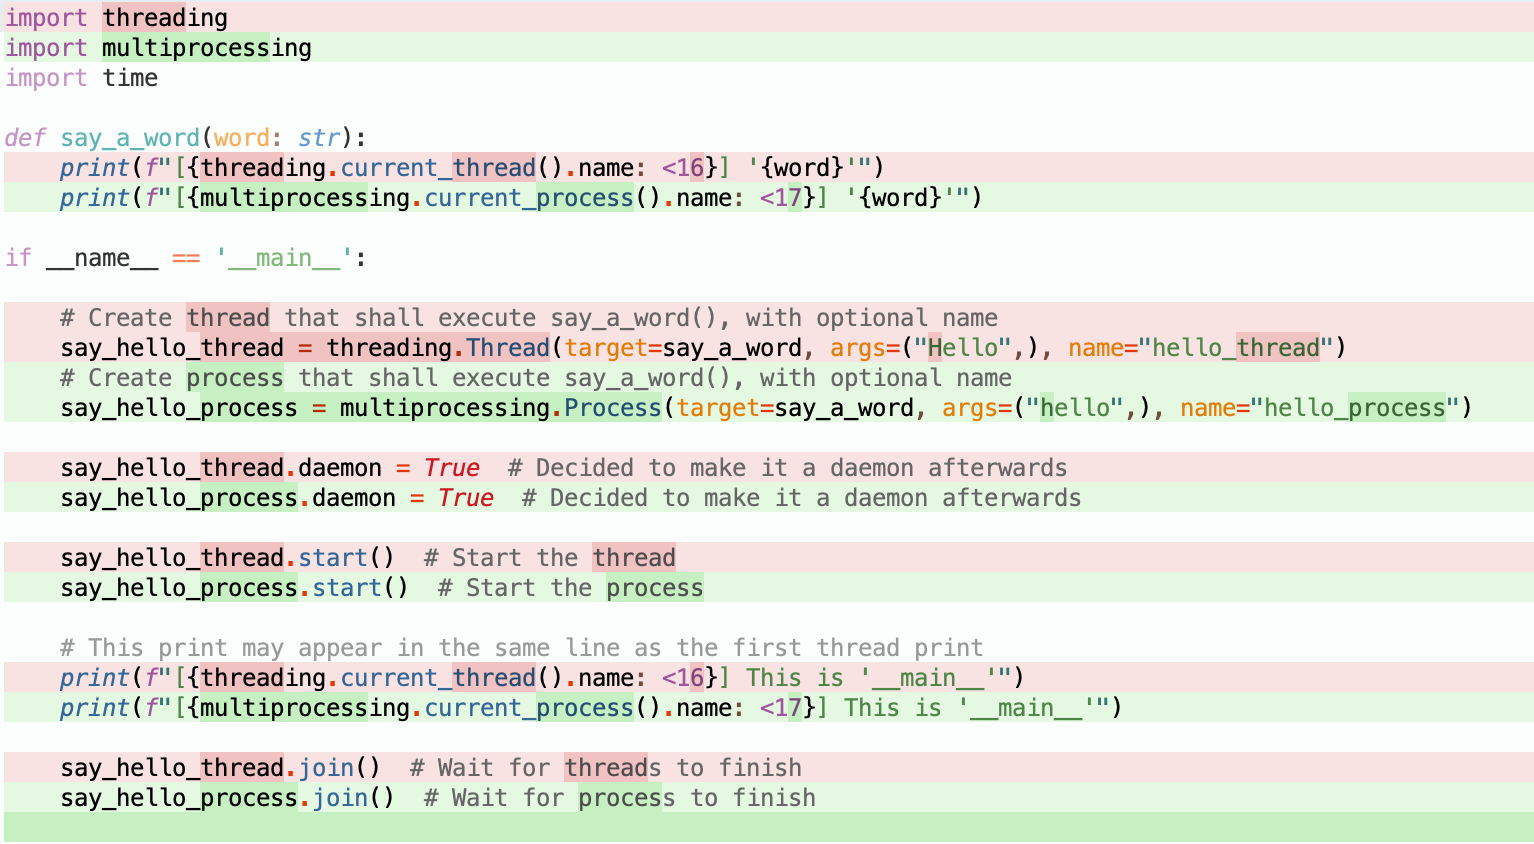
\includegraphics[height=0.7\textheight]{thread_vs_process.png}
		\caption{Der Diff zwischen dem Threading und Multiprocessing Beispiel}
	\end{figure}
\end{frame}



\begin{frame}[fragile]{Multiprocessing das 1:1 Replacement für Threading?}
	\begin{itemize}
		\item Das Hauptproblem ist der \tb{unterschiedliche Adressraum}.
		\item[] Hierdurch können \tb{keine geteilten} Lese- und Schreibvorgänge auf dem selben Objekt durchgeführt werden.
	\end{itemize}
\end{frame}



\begin{frame}[fragile]{Variablen und Prozesse}
	\begin{itemize}
		\item Die in einem Prozess ausgeführte Funktion nimmt \tb{alle globalen Variablen} ihres Scopes mit.
		\item[] Von diesen wird eine \tb{Kopie} angelegt.
		\item Verändert ein Prozess seine Version dieser Variable, bekommen die anderen Prozesse dies nicht mit.
		\pause
		\item Der erzeugende Prozess wird als \tb{parent} bezeichnet, der erzeugte Prozess als \tb{child}.
	\end{itemize}
\end{frame}


%TODO: Super mario meme
\begin{frame}[fragile]{Kommunikation zwischen Prozessen}
	\begin{itemize}
		\item Zwischen Prozessen können sog. \tb{Pipes} erzeugt werden.
		\pause
		
		\item Des Weiteren gibt es u.A. Message \tb{Queues}, Semaphoren.
		\pause
        \item \tb{Signale}
		\item Es kann geteilter Speicher (\pp{Value}, \pp{Array}) erstellt werden.
		\item Eine Kommunikation über Sockets (als Netzwerkkommunikation) ist auch möglich
	\end{itemize}
\end{frame}


\begin{frame}[fragile]{Pipe}
	\begin{itemize}
		\item Eine \pp{multiprocessing.Pipe} ist eine Verbindung zwischen \tb{zwei Prozessen}.
		
		\pause
		\item Man kann sie sich wirklich wie ein Rohr zwischen zwei Prozessen vorstellen. 
		\item[] Auf beiden Seiten kann \tb{gelesen und geschrieben} werden.
		
		\pause
		\item Nachrichten können auf der empfangenden Seite aus der Pipe ausgelesen werden, so lange die Pipe auf der empfangenden Seite offen ist.
		\item Eine Pipe kann so lange beschrieben werden, wie sie auf der empfangenden Seite noch offen ist.
		
		\pause
		\item Eine Pipe sollte \tb{geschlossen} werden, wenn sie nicht mehr benötigt wird.
	\end{itemize}
\end{frame}


\begin{frame}[fragile]{Pipe in python}
	\begin{itemize}
		\item Die Rückgabe von \pp{multiprocessing.Pipe()} ist ein \tb{Tupel} aus\\ \pp{multiprocessing.connection.Connection}\footnote{Die Connection hat ein Interface analog zu einem Socket.}\footnote{Um sie zu Typehinten muss \texttt{
        multiprocessing.connection} oder \texttt{Connection} direkt importiert sein.}, die \tb{je eine Seite} repräsentiert.
    
    	\pause
		\item Mit \pp{.send()} kann geschrieben und mit \pp{.recv()} gelesen werden.
		\item[] Daten werden durch \pp{pickle} serialisiert übertragen.
		\item[] Dies ist bei hoher Datenrate spürbar langsam.
		
		\pause
		\item Mit \pp{.poll(timeout=...)} kann abgefragt werden, ob Daten in der Pipe vorliegen.
		
		\pause
		\item Pipes werden mit \pp{.close()} geschlossen, wenn sie nicht mehr gebraucht werden.
		\item[] Wird versucht in eine Pipe zu schreiben, die auf der anderen Seite geschlossen ist, gibt es den \pp{BrokenPipeError}.
	\end{itemize}
\end{frame}


\begin{frame}[fragile]{Pipes minimal Beispiel}
	\begin{lstlisting}[language=pytiny]
def sender(pipe: multiprocessing.connection.Connection):
    messages_to_send = ["Message 1", "Message 2", "Message 3"]
    for msg in messages_to_send:
        pipe.send(msg)   # put message to pipe
        time.sleep(0.5)  # Add a delay between messages

if __name__ == "__main__":

    parent_side, child_side = multiprocessing.Pipe()  # create pipe

    sender_process = multiprocessing.Process(target=sender, args=(parent_side,)).start()

    while True:
        if child_side.poll(timeout=2):  # try to get a new message, timeout after two seconds
            received_data = child_side.recv()  # read data if available
            print("Received:", received_data)
        else:
            print("No more messages.")
            break
	\end{lstlisting}
\end{frame}



\begin{frame}[fragile]{Queues in Python}
	\begin{itemize}
		\item Die \pp{multiprocessing.Queue}\footnote{\url{https://docs.python.org/3/library/multiprocessing.html\#multiprocessing.Queue}} ist prozesssicher und und dient zum \tb{Austausch} von Inhalten zwischen \tb{mehreren Prozessen}\footnote{Insbesondere sind mehr als zwei möglich.}.
		
		\pause
		\item In eine Queue können alle Prozesse \tb{schreiben und lesen}.
		\pause
		\item Hinweis: Analog zur multiprocessing Queue gibt es \pp{queue.Queue}, welche threadsafe ist und \pp{asyncio} bringt ebenfalls seine eigene Queue mit.
		
		\pause
		\item[] Die \glqq \tb{normale}\grqq~ (und effizientere Queue) heißt \pp{collections.deque}.
	\end{itemize}
\end{frame}


\begin{frame}[fragile]{Queues - Beispiel}
	\begin{lstlisting}[language=pytiny]
def producer(queue):
    messages_to_send = ["Message 1", "Message 2", "Message 3"]
    for msg in messages_to_send:
        queue.put(msg)
        time.sleep(1)  # Add a delay between messages
    queue.put(None)    # Signal the end of messages

if __name__ == "__main__":
    queue = multiprocessing.Queue()

    producer_process = multiprocessing.Process(target=producer, args=(queue,))
    producer_process.start()

    while True:
        message = queue.get()
        if message is None:  # None is explicitly used to signal the end of messages
            break
        print("Received:", message)

    producer_process.join()
	\end{lstlisting}
\end{frame}

\begin{frame}[fragile]{Ein Blick unter die Haube: pickle}
	\begin{itemize}
		\item Das \pp{pickle}-Modul kann \tb{Objekte als Byte-Stream serialisieren}.
		
		\pause
		\item[] Dieser enthält das \tb{konkrete Objekt} mit seinen Daten.
		\pause
		
		\item[] Streams können dann via \pp{Pipe} an andere \tb{Prozesse} geschickt werden.
		
		\pause
		\item Bedigung: Die serialisierte Klasse muss in dem importierenden Modul \tb{bekannt} sein.
		\item \tb{Globale} Variablen werden aus dem \tb{alten} Scope mitgebracht.
		\item \tb{Klassenvariablen} u.Ä. werden aus dem \tb{aktuellen} Scope übernommen.
		
		\pause
		
		\item Es ist möglich, \tb{Dumps} zu erstellen, welche \tb{beliebigen} Code während des Ladens ausführen. Dies ist insbesondere für bösartige Entwickler nützlich\footnote{Für das Absichern wird Sining mit hmac (\url{https://docs.python.org/3/library/hmac.html\#module-hmac}) oder json-Serialisation empfohlen.}.
	\end{itemize}
\end{frame}


\begin{frame}[fragile]{Serialisieren mit pickle}
	\begin{lstlisting}[language=pytiny]
import pickle


class PickleClass:
    class_var = "cv"
    def __init__(self, data):
        self.data = data

    def say_global_var_x(self):
        print(x)

    def say_data(self):
        print(self.data)

x = 42
obj = PickleClass(69)

# file needs to be opened in byte mode
with open("pkl_file.pkl", "wb") as f:
    pickle.dump(obj, f)		
	\end{lstlisting}
\end{frame}


\begin{frame}[fragile]{Deserialisieren mit pickle}
	\begin{lstlisting}[language=pytiny]
import pickle

from pickle_dump import PickleClass

x = 41

PickleClass.class_var = "newcv"

with open("pkl_file.pkl", "rb") as f:
    obj = pickle.load(f)

obj.say_global_var_x()  # >> 42
obj.say_data()          # >> 69
print(obj.class_var)    # >> "newcv"

x = 43
obj.say_global_var_x()  # >> 42
		
	\end{lstlisting}
\end{frame}


% TODO: ist das hier alles universell korrekt?
\begin{frame}[fragile]{Signale}
	\begin{itemize}
		\item \tb{Signale} sind ein ganzes Thema für sich, wir sprechen sie hier sehr oberflächlich an.
		
		\pause
		
		\item Prozesse können über Signale \tb{kommunizieren}.
		
		\pause
		
		\item Jeder Prozess kann einen \tb{Signalhandler} registrieren, welcher ein Verhalten bei einem Signal definiert.
		\item[] In Python können sie über das \pp{signal}-Modul registriert werden.
		
		\pause
		
		\item Signale werden \tb{unabhängig vom Programmfluss} behandelt, sobald sie ankommen.
		
		\pause
		
		\item Relevante Signale\footnote{Signale sind auch in dem signal-Modul vordefiniert.} sind \pp{SIGINT}\footnote{Wird z.B. bei Ctrl+C geschickt.}, \pp{SIGTERM}\footnote{Verschickt kill Command per Default.} und \pp{SIGHUP}\footnote{Das Signal, dass das Terminal, welches den Prozess ausführt geschlossen wurde.}.
		\item FunFact: \pp{SIGKILL} kann nicht abgefangenen werden.
		
	\end{itemize}
\end{frame}


\begin{frame}[fragile]{Signale minimal Beispiel}
	\begin{lstlisting}[language=pytiny]
def child_process():
    def child_signal_handler(sig, frame):
        print("Received SIGINT in child process. Exiting gracefully.")
        exit(0)

    # Set up the signal handler for SIGINT (Ctrl+C) in the child process
    signal.signal(signal.SIGINT, child_signal_handler)

    while True:
        print("Child process is running.")

if __name__ == "__main__":
    child_proc = multiprocessing.Process(target=child_process)
    child_proc.start()

    time.sleep(3)
    print("Sending the 'Ctrl+C' Signal from main to child process.")
    child_proc.terminate()
    child_proc.join()
	\end{lstlisting}
\end{frame}


\begin{frame}[fragile]{Signale - Der brutale Weg}
	\begin{itemize}
		\item Über das \pp{os}-Modul kann ein nicht reagierendes Kind \tb{gewaltvoll} gekillt werden.
		
		\pause
		
		\item Dies gibt dem Prozess \tb{keine} Chance, kontrolliert zu stoppen, um z.B. Daten zu sichern.
	\end{itemize}
	\begin{lstlisting}[language=pytiny]
def infinite_loop():
    while True:
        print("I'm unstoppable! - Wheeee!")

# Start child
child = multiprocessing.Process(target=infinite_loop)
child.start()

# Wait for a few seconds
time.sleep(3)

# Kill the child using SIGKILL
print("That's enough...")
os.kill(child.pid, signal.SIGKILL)
print(f"No you're not. ~parent")
	\end{lstlisting}
\end{frame}


\begin{frame}[fragile]{Multiprocessing einfach gemacht}
	\begin{itemize}
		\item Python hat viel des Setups über Prozesse weg \tb{abstrahiert}.
		
		\pause
		\item Python bietet \tb{Prozess-Pools}.\footnote{\url{https://docs.python.org/3/library/multiprocessing.html\#module-multiprocessing.pool}}
		\item[] Ein \pp{Pool} ist eine Menge an n-Prozessen, auf welche die Aufgaben dann \tb{automatisch verteilt} werden.
		\pause
		
		\item Auf den Pools können \tb{Maps} genutzt werden. Eine dieser Maps ist die \pp{starmap}.
		\item[] Diese nimmt ein iterierbares Objekt aus iterierbaren Argument-Mengen entgegen und gibt die Liste aus Return-Werten zurück.
		
		\pause
		\item Nur weil ein Pool über n-Prozesse verfügt, bedeutet dies nicht, dass immer alle n-Prozesse genutzt werden.
	\end{itemize}
\end{frame}


\begin{frame}[fragile]{Starmap}
	\begin{lstlisting}[language=pytiny]
import multiprocessing
import time


def worker_function(a, b):
    result = a + b
    print(f"[{multiprocessing.current_process().name: <17}] {a+b = }")
    time.sleep(2)  # sleep to better visualize the result
    return result

if __name__ == "__main__":
    # List of argument tuples
    arguments = [(1, 2), (3, 4), (5, 6), (7, 8)]

    # Create a pool of processes with four processes
    with multiprocessing.Pool(processes=4) as pool:
        results = pool.starmap(worker_function, arguments)

    print("Results:", results)

	\end{lstlisting}
\end{frame}


\begin{frame}{Pool.apply\_async}
	\begin{itemize}
		\item \pp{Pool.apply_async}\footnote{Achtung: Das bekannte \texttt{kwargs} heißt hier \texttt{kwds}.} ist ein gutes \glqq Drop-In\grqq~ \tb{Replacement} für Berechungen z.B. innerhalb eines bereits \tb{existierenden Loops}, ohne viel Umbau.
		
		\pause
		
		\item Statt die Inputs explizit für eine \pp{map} oder \pp{starmap} vorzubereiten, Berechnung an dieser Stelle mit den aktuellen Parametern gescheduled werden.
		
		\pause
		
		\item Die Tasks werden \tb{non-blocking} gescheduled. Das Return-Value ist ein \pp{AsyncResult}.
		\item[] Das Ergebnis kann mit \pp{.get()} (blockierend) abgerufen werden.
		
		\pause
		
		\item $\rightarrow$ Es ist notwending Track über die \tb{geschedulten Prozesse} zu behalten, wenn der \tb{Rückgabewert} von Relevanz ist.
	\end{itemize}
\end{frame}


\begin{frame}[fragile]{Pool.apply\_async - Beispiel}
	\begin{lstlisting}[language=pytiny]
def parabola(x, a=1, b=0):
    return a * x**2 + b

pool = Pool(processes=4)
inputs = list(range(20))
tasks = []

for i in inputs:
    # generate all the tasks from line that was the previous calculation
    # note the creation of kwargs via dict() as easier drop-in from previous structure
    task = pool.apply_async(parabola, args=(i,), kwds=dict(a=i, b=i))  
    results.append([task, (i, i, i)])

# Get the return values from the asynchronous tasks in the order they were submitted
for task, (a, x, b) in tasks:
    output = task.get()  # note: get is blocking
    print(f"{a}*{x}**2+{b} = {output}")

pool.close()  # don't accept any new tasks, worker-processes will exit when queue is done
pool.join()   # wait for worker-processes to exit
	\end{lstlisting}
\end{frame}


\begin{frame}[fragile]{Hinweis: RuntimeError}
	\begin{itemize}
		\item Währen der Erstellung eines Prozesses kann \tb{kein anderer} gespawnt werden.
		\pause
		
        \item Es kommt ein langer, etwas kryptischer \pp{RuntimeError}, wenn Prozesse in der Main-Datei, \tb{außerhalb} einer Funktion und der \pp{__main__}-Abfrage der gespawnt werden.
		\item Begründung: Wird ein neuer Prozess erstellt, wird das Modul erneut in den neuen Prozess \tb{geladen} und damit ausgeführt.
		
		
		\item[] Dabei kann - \tb{quasi rekursiv} - versucht werden Prozesse zu spawnen. Dies wird von Python durch den Fehler verhindert.
		
		\pause
		\item Die Lösung ist es, das \tb{Erstellen} einfach hinter die \pp{__main__}-Abfrage zu schreiben.
		\item[] Denn der \tb{Wert} von \pp{__name__} ist in Kind-Prozessen \pp{__mp_main__} statt \pp{__main__}.
	\end{itemize}
\end{frame}


\begin{frame}[fragile]{Potentielle Deadlocks sinnvoll debuggen}
	\begin{itemize}
		\item Es ist schwer den \tb{Punkt} zu finden, an welchem ein Programm hängen könnte.
		
		\pause
		
		\item Python bietet das Modul \pp{faulthandler}\furl{https://docs.python.org/3/library/faulthandler.html} zum \tb{Untersuchen} von lang dauernden Operationen.
		
		\pause
		
		\item \pp{faulthandler} bietet Wege Pythons \tb{Traceback} geordnet zu dumpen.
		
		\pause
		
		\item Bei Erhalt eines \tb{Signals}\footnote{Mögliche Signale, um ein Traceback auszulösen: \texttt{SIGSEGV, SIGFPE, SIGABRT, SIGBUS, SIGILL}} dumped es das aktuelle Traceback.
		\item[] Das Modul kann mit \pp{.enable()} aktiviert werden.
		
		\pause
		
		\item Alternativ kann ein Dump \tb{manuell} gescheduled werden.
	\end{itemize}
	\begin{lstlisting}[language=pytiny]
# end programm in five seconds if it doesn't end on it's own - print traceback to terminal
faulthandler.dump_traceback_later(5, exit=True, file=sys.stdout)
function_that_takes_forever_maybe_because_of_deadlock()
\end{lstlisting}

	
\end{frame}


% TODO: Prozesse beenden


\begin{frame}[fragile]{Interesse geweckt?}
	Die Vorlesung \tb{Systemnahe Programmierung} behandelt genau diese Themen und ist sehr empfehlenswert!\\
\end{frame}



\framecardfragen


\section{Iteratoren}

%Special methods
%Functional
% Generator expressions

% consume
%loops


\subsection{In Python}

\begin{frame}[fragile]{Ein kleines Beispiel}

    \begin{lstlisting}[language=pytiny]
my_list = [1, 2, 3, 4]

iterator = iter(my_list)

print(next(iterator))
print(next(iterator))

print("----")

for i in iterator:
    print(i)

# Output:
# 1
# 2
# ----
# 3
# 4
    \end{lstlisting}

\end{frame}

\begin{frame}[fragile]{Klassen basiert}

    Ein Iterator ist eine Klasse die, die \tb{special Methods} \pp{__iter()__} und \pp{__next()__} implementiert.

    \medskip

    \begin{lstlisting}[language=pytiny]
from typing import Any

class ListIterator:
    def __init__(self, lst: list[Any]):
        self.lst = lst
        self.index = -1

    def __iter__(self):
        return self

    def __next__(self) -> any:
        self.index += 1
        if self.index < len(self.lst):
            return self.lst[self.index]
        raise StopIteration

    \end{lstlisting}

\end{frame}

\begin{frame}[fragile]{Funktions basiert}

    Mithilfe von \pp{yield} können Funktionen zu Iteratoren transformiert werden. Diese Funktionen werden \tb{Generator Funtktionen} gennant.

    \medskip

    \begin{lstlisting}[language=pytiny]
from typing import Any

def list_iterator(lst: list[Any]) -> Generator[int, None, None]:
    indx = 0
    while indx < len(lst):
        yield lst[indx]

    \end{lstlisting}

\end{frame}

\begin{frame}[fragile]{Generator Expressions}

    \tb{Generator Expression} können ebenfalls einen Iterator erzeugen.
    
    \medskip

    \begin{lstlisting}[language=pytiny]
my_list = [1, 2, 3, 4]

it = (i for i in my_list)

next(it)  # >> 1
next(it)  # >> 2
    \end{lstlisting}

Das ist nur möglich, wenn das zu iterierende Objekt selbst \tb{Iterable} ist.

\end{frame}

\begin{frame}[fragile]{Unendliche Iteratoren}

    Falls der Iterator \tb{keine Abbruchbedingung} hat, wird er zu einem unendlichen Iterator. Diese können praktisch sein, um Streams zu verarbeiten.

    \begin{lstlisting}[language=pytiny]
def inf_iterator():
    counter = 0
    while True:
        yield counter
        counter += 1

it = inf_iterator()

next(it)  # >> 0
next(it)  # >> 1
    \end{lstlisting}

\end{frame}

\begin{frame}{Iterable vs Iterator}
    
    In Python Objekt kann ein \tb{Iterator} oder ein \tb{Iterable} sein.
    \begin{itemize}
        \item Ein \tb{Iterable} repräsentiert ein Objekt, über das iteriert werden kann. Ein Iterable implementiert \pp{__iter__()}.
        \item Ein \tb{Iterator} implementiert die \pp{__iter__()} und \pp{__next__()} Methode, dabei gibt \pp{__next__()} immer das nächste Element zurück.
    \end{itemize}

    Iterables \tb{produzieren} Iteratoren. Iteratoren \tb{durchlaufen} einen Strom von Daten.

\end{frame}

\begin{frame}{Ein paar funfacts}
    \begin{itemize}
        \item Ein Iterator kann nur \tb{einmal} durchlaufen werden. Danach ist er leer und muss neu erstellt werden.
        \item Da nur die \pp{__next__()} Methode existiert, kann ein Iterator nur \tb{vorwärts} durchlaufen werden und es kann niemals der vorherige Wert abgerufen werden.
        \item Alle Operationen auf Iteratoren werden \tb{\glqq lazy \grqq evaluated}. Das heißt, ein Ergebnis wird genau dann berechnet, wenn es benötigt wird.
    \end{itemize}
\end{frame}

\begin{frame}[fragile]{Iteratoren anwenden}
    Mithilfe von Iteratoren können Konzepte der \tb{funktionelle Programmierung} umgesetz werden.

    \begin{lstlisting}[language=pytiny]
nums1 = (1, 2, 3, 4)
nums2 = (6, 7, 8, 9)
nums3 = (10, 11, 6, 9)

my_list = [1, 3, 4, None, 7, 8]

# Checks if any of the values in iterable are Truthy
print(all(my_list))  # >> false da bool(None) false

# filters every element which returns true when given into bool
list_filtered = filter(bool, my_list)  # >> [1, 3, 4, 7, 8]
zipped = zip(nums1, nums2, nums3, list_filtered)  # >> [(1, 6, 10, 1), (2, 7, 11, 3), (3, 8, 6, 4), (4, 9, 9, 7)]
mapped = map(sum, zipped)  # >> [18, 23, 21, 29]
filtered = filter(lambda x: x >= 20, mapped)  # >> [23, 21, 29]
    \end{lstlisting}
\end{frame}

% Itertools:
% Beispiel, map, filter, zip, all
% islice, pemutations, combinations


% Functools
% partial, singedispatch, wraps
\begin{frame}{Itertools}
    Die Python Standardbibliothek \pp{itertools}\footnote{\url{https://docs.python.org/3/library/itertools.html}} stellt weitere Funktionalität auf Iteratoren zur Verfügung.

    \begin{itemize}
        \item Mit \pp{islice} ist es möglich, nur einen bestimmten \tb{Abschnitt} eines Iterators zu betrachten.
        \item \pp{permutations} stellt alle möglichen \tb{Permutationen} gegebener Länge eines Iterators zur Verfügung.
        \item \pp{combinations} stellt alle möglichen \tb{Kombinationen} von gegebener Länge eines Iterators zur Verfügung.
    \end{itemize}
\end{frame}

\begin{frame}{Functools}
    Die Python Standardbibliothek \pp{functools}\footnote{\url{https://docs.python.org/3/library/functools.html}} stellt weitere Fuktionalität auf Funktionen zur Verfügung-.

    \begin{itemize}
        \item Mit \pp{partial} kann aus einer Funktion eine \tb{neue} erstellt werden, wobei einige der Parameter festgelegt werden. Dadurch  nimmt die neue Funktion nur noch einen \tb{Teil} der vorher erforderlichen Parameter und wurde bereits partiell mit Argumenten gefüllt.
        \item \pp{singledispatch} erlaubt \tb{Funktonsüberladung}. 
        \item \pp{wraps} ermöglicht es, die Signatur einer Wrapper Funktion auf die der gewrappten Funktion zu setzen.
    \end{itemize}
\end{frame}

\framecardfragen


\section{logging}
\begin{frame}{logging - Motivation}
	\begin{itemize}
		\item Das \glqq Loggen\grqq~ auf das Terminal kommt mit einigen Problemen:
		\item[] \begin{itemize}
			\item Prints sind in der Regel sehr chaotisch und nicht einheitlich formattiert.
			\item Je nach Umgebung kann stdout des Programms nicht so einfach eingesehen werden (Hintergrundtask und geschlossene SSH-Verbindung).
			\item Das Terminal kann irgendwann die obersten Zeilen des Outputs abschneiden.
			\item Im Allgemeinen nicht gut zu durchsuchen.
		\end{itemize}
		\item Es wäre wünschenswert die Logs in einer strukturierteren, persitenten Form einsehbar zu haben.
		
	\end{itemize}
\end{frame}


\begin{frame}{logging - Konzept}
	\begin{itemize}
		\item Logging besteht aus dem \tb{strukturierten Dokumentieren} von Ereignissen, welche innerhalb des Programms auftreten.
		\item Die geloggten Nachrichten sollen \tb{einheitlich formattiert} sein.
		\item[] Hierbei sollte die Nachricht möglichst viel Kontext enthalten.
		\item[] $\rightarrow$ Zeit des Events, Funktion / Modul, Thread, ...
		\item Diese Nachrichten sollten an einem persistenten, \tb{zentralen Ort} gesammelt werden.
		\item[] Hierfür eignet sich in der Regel die Nutzung einer Datei.
		\item Im Allgemeinen wird bei den Log-Nachrichten zwischen \tb{verschiedenen Leveln} von Wichtigkeit unterschieden: \pp{debug}, \pp{info}, \pp{warning}, \pp{error} und \pp{critical}
		\item Es soll ein \tb{Relevanz-Level wählbar} sein, ab welchem Nachrichten geloggt werden.
		
	\end{itemize}
\end{frame}

\subsection{Pythons logging modul}
\begin{frame}{Das logging-Modul\footnote{Dieses Kapitel war bereits in Tag 3 enthalten, wurde aus Zeitgründen dort nicht behandelt. Daher ist es hier erneut enthalten.}}
	\begin{itemize}
		\item Python liefert das eigene Modul \pp{logging}.
		\item Dieses enthält alles benötigte, um \tb{sinnvolles} Logging nutzen zu können.
		\item Wir betrachten das \tb{fortgeschrittene} Logging mit Hilfe der \pp{Logger}-, \pp{Handler}- und \pp{Formatter}-Klassen.
	\end{itemize}
\end{frame}

\begin{frame}[fragile]{logging - Der Logger}
	\begin{itemize}
		\item Die \tb{zentrale Klasse} des Moduls ist der \pp{Logger}.
		\item Der Logger ist das Objekt welches die \tb{Methoden zum melden von Nachrichten} zur Verfügung stellt, welche vom Code aufgerufen werden.
		\item Er evaluiert, ob die Nachricht dem gesetzten Log-Level oder höher entspricht.
		\item Ist die \tb{Nachricht von Relevanz}, gibt er den \pp{LogRecord}\footnote{\url{https://docs.python.org/3/library/logging.html\#logging.LogRecord}} an die registrierten \pp{Handler} weiter. 
		\item Logger werden nicht direkt, sondern \tb{über} \pp{getLogger()} \tb{instanziiert}.
		\item[] Dies registriert das Objekt global in der Library. \item[] $\rightarrow$ Andere Module können sich damit die selbe (konfigurierte) Instanz holen.
		
		
	\end{itemize}
	\begin{lstlisting}[language=pytiny]
		import logging
		logger = logging.getLogger('my_logger')
	\end{lstlisting}
\end{frame}


\begin{frame}{logging - Die Handler}
	\begin{itemize}
		\item Ein \tb{Handler} nimmt Nachrichten in Form eines \pp{LogRecord} entgegen.
		\item Dann prüft er, ob die Nachricht seinem eigenen \tb{gesetzten Log-level} entspricht.
		\item Im Anschluss ruft er seine \pp{emit()}-Methode\footnote{\url{https://docs.python.org/3/library/logging.html\#logging.Handler.emit}} auf, welche den Record mit Hilfe eines \pp{Formatters} formattiert und anschließend meldet.
		\item \tb{Relevante Handler}\footnote{\url{https://docs.python.org/3/library/logging.handlers}} sind:
		\item[] \begin{itemize}
			\item \pp{StreamHandler}: Schreibt auf einem \tb{Stream}, wie \pp{stdout} aus.
			\item \pp{FileHandler}: Schreibt in gegebene \tb{Datei}.
			\item \pp{TimedRotatingFileHandler}: Schreibt in Datei, die in  \tb{Intervallen} wechselt.
			\item \pp{SysLogHandler}: Schreibt in einen \tb{Unix-Syslog}.
		\end{itemize}
	\end{itemize}
\end{frame}


\begin{frame}[fragile]{logging - Formatter}
	\begin{itemize}
		\item Das Formatter-Objekt\footnote{\url{https://docs.python.org/3/library/logging.html\#formatter-objects}} konvertieren das \pp{LogRecord} in eine \tb{lesbare Form}.
		\item Dies inkludiert das automatische \tb{Hinzufügen von Informationen}\footnote{Alle verfügbaren Informationen: https://docs.python.org/3/library/logging.html\#logrecord-attributes}.
	\end{itemize}
	\begin{lstlisting}[language=pytiny]
		formatter_string = "[{asctime}] [{levelname}][{threadName}][{module}.{funcName}] {message}"
		formatter = logging.Formatter(formatter_string, style="{")
		\end{lstlisting}
		\begin{itemize}
			\item Im Programm muss dann nur noch die \pp{message} gemeldet werden.
		\end{itemize}
		\begin{lstlisting}[language=pytiny]
			logger.warning("This is a warning")
			# >> [2023-09-06 20:08:24,847] [WARNING] [MainThread][logging_example.<module>] Hello world
		\end{lstlisting}
	\end{frame}
	
	
	\begin{frame}{logging - Ablauf Diagram}
		\begin{figure}
			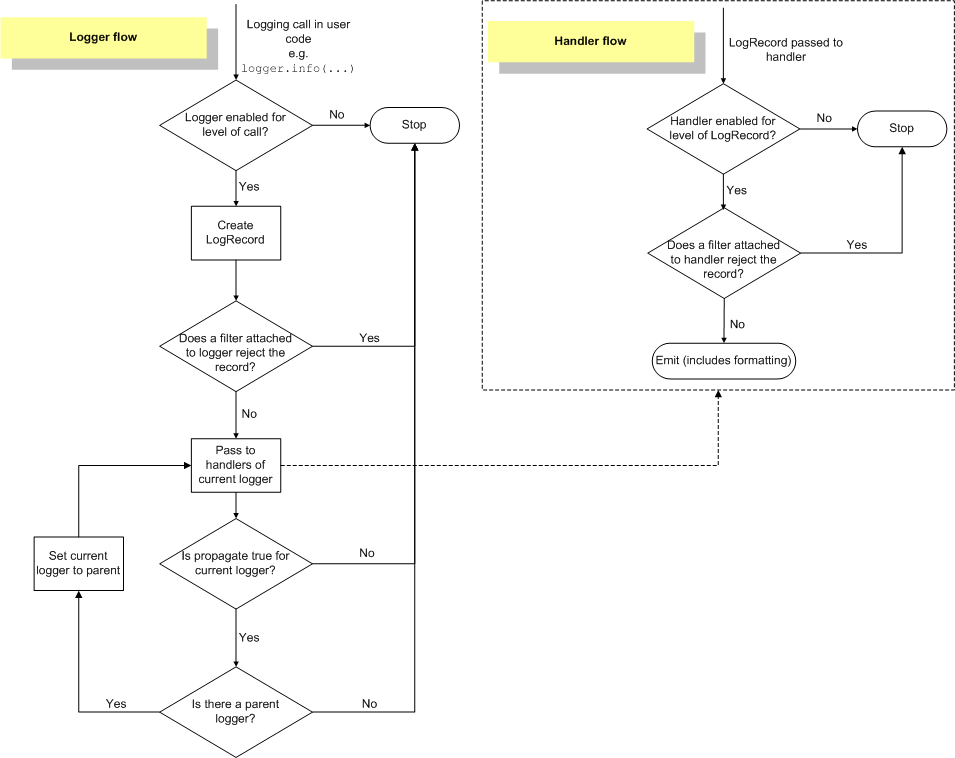
\includegraphics[height=0.7\textheight]{images/03_logging_flow.png}
			\caption{\url{https://docs.python.org/3/howto/logging.html\#logging-flow}}
		\end{figure}
	\end{frame}
	
	
	\begin{frame}[fragile]{logging - Ein ziemlich gutes Beispiel-Setup}
		\begin{lstlisting}[language=pytiny]
			formatter = logging.Formatter("[{asctime}] [{levelname}] [{threadName}][{module}.{funcName}] {message}", style="{")
				
				# init one normal filehandler and a stream-handler for stdout
				file_logger = logging.FileHandler("events.log")
				file_logger.setLevel(logging.DEBUG)
				file_logger.setFormatter(formatter)
				
				console_logger = logging.StreamHandler()
				console_logger.setLevel(logging.WARNING)
				console_logger.setFormatter(formatter)
				
				logger = logging.getLogger("my_logger")
				# set logger to lowest, the handlers can then decide on their own
				logger.setLevel(logging.DEBUG)
				
				logger.addHandler(console_logger)
				logger.addHandler(file_logger)
			\end{lstlisting}
		\end{frame}

\framecardfragen

\end{document}

